 \documentclass[fleqn,10pt]{wlscirep}
\usepackage[utf8]{inputenc}
\usepackage[T1]{fontenc}
\usepackage{bm}
\usepackage{caption}
\usepackage{subcaption}
%\usepackage{natbib}
\graphicspath{{figures/}}


\title{Molecular transport in human pial perivasculature}

\author[1,x]{Rami Masri}
\author[1,x]{Miroslav Kuchta}
\author[1,x]{Marius Causemann}
\author[1,*]{Marie E. Rognes}
\affil[1]{Department of Numerical Analysis and Scientific Computing, Simula Research Laboratory, Oslo, Norway}
\affil[x]{Author order to be discussed.}
\affil[*]{meg@simula.no}

\newcommand{\rami}[1]{\textcolor{blue}{#1}}


%\affil[+]{these authors contributed equally to this work}

%\keywords{Keyword1, Keyword2, Keyword3}

\begin{abstract}
\end{abstract}
\begin{document}

\flushbottom
\maketitle
% * <john.hammersley@gmail.com> 2015-02-09T12:07:31.197Z:
%
%  Click the title above to edit the author information and abstract
%
\thispagestyle{empty}

\section*{Introduction}

Molecular transport in perivascular spaces (PVSs) is established as a key pathway for human brain clearance and delivery. Previous studies indicate that molecules move rapidly in the subarachnoid space (SAS) and in PVSs surrounding pial arteries. Here, we aim to model and study this transport in a full pial perivascular and/or vascular network embedded in the SAS.  

\begin{itemize}
\item Vinje et al~\cite{vinje2021brain} and references therein illustrates the location and characteristics of human pial perivascular spaces.
\item Mestre et al~\cite{mestre2022periarteriolar} study the properties of pial perivascular spaces in detail in mice.
\item Mestre et al~\cite{mestre2018flow} measure and characterize pial perivascular transport and estimate flow magnitudes (in mice).
\item Bakker and coauthors studied perivascular spaces at the brain surface in a series of papers. They found that paravascular spaces (in particular periarterial spaces) represented low-resistance pathways~\cite{bedussi2017paravascular}, in communication with the surrounding CSF-filled subarachnoid spaces~\cite{bedussi2018paravascular}.
\item Bollman et al~\cite{bollmann2022imaging} image the human pial vasculature at high resolution (7T).
\item Hornkjøl et al~\cite{hornkjol2022csf} model CSF flow and solute transport in the human SAS and brain parenchyma. 
\item Mardal et al~\cite{mardal2022mathematical} give a succinct introduction to MRI-based computational brain modelling. 
\end{itemize}

\section*{Methods}

\subsection*{Meshing}

\cite{hodneland2019new} developed a method to image the brains' microvasculature based on time-of-flight (ToF) and quantitative susceptibility mapping (QSM) to identify arterial and venous networks.
We derive a detailed tetrahedral mesh of both the parenchyma and the surrounding CSF-filled spaces alongside a network representation of the vasculature from the anatomical data provided therein. 

\paragraph{3D domain}

We merge the white and grey matter masks provided by \cite{hodneland2019new} to extract the pial surface. As no data on the CSF-filled spaces is available, we smooth and extend the pial surface by about 5\,mm to obtain an approximation of the SAS and include the inner fluid-filled cavities such as the ventricular system. 
Finally, we generate a tetrahedral mesh of both compartments using the fTetWild meshing algorithm \cite{hu2020fast}.

\paragraph{Vessel networks}

We skeletonize the binary masks of both the arterial and venous network using Kiminaro \cite{william_silversmith_2021_5539913} and obtain networks consisting of centerline and radius information of all detected vessels. The resulting networks are further smoothened using a spline interpolation technique and the nodes with lowest z-coordinate are identified as the networks' root nodes.

\subsection*{Geometries and domains}

The computational domain $\Omega$ is defined by the union of the SAS $\Omega_{\rm sas}$ and brain parenchyma $\Omega_{\rm brain}$. The thin pia membrane encloses the brain, and thus the pial surface (of the brain) defines the SAS-brain interface $\Gamma_{\rm pia}$. A network of blood vessels are embedded in the SAS, potentially very near to or on the pial surface. We assume that a network of idealized (annular or semi-annular) perivascular spaces surround the vasculature. We represent the vasculature and associated perivasculature by a network of one-dimensional curves $\Gamma$ representing the network centerlines equipped with inner $R_1$ and outer $R_2$ radius information. 

Surface representations of the outer SAS boundary, pial membrane, and delimiters of other CSF-filled spaces such as the lateral ventricles, third and fourth ventricle, and aqueduct are extracted from MR-images of human subject(s), see e.g. the pipeline described by Hornkjøl et al.~\cite{hornkjol2022csf}. From these surface representations, we create volumetric meshes of the SAS and brain using SVMTK~\cite{mardal2022mathematical}. 

\begin{itemize}
    \item To discuss: How to generate subject-specific representations of the pial/SAS vasculature? Can we use contrast MRI? Can we use time-of-flight images? What are the right tools? Do any data sets already exist? 
    \item How to add radius information to vasculature representation? Do we need more information as well?
\end{itemize}


\begin{figure}
\caption{(A) Illustration of the location of pial vasculature and subarachnoid space. (B) Conceptual illustration of the vascular, perivascular, SAS and cortex domains (cross-section and lateral view).}
\label{fig:concept}
\end{figure}

\subsection*{Multi-dimensional transport model}

We consider a time-dependent convection-diffusion model~\cite{masri2023modelling} of a solute concentration $c$ in the network representing the pial vasculature and surrounding perivascular spaces $\Lambda$ and the surrounding three-dimensional SAS-brain domain $\Omega$ (Fig.~\ref{fig:concept}). 

\subsection*{Diffusion}
We use the diffusion coefficient $D_{\rm gad}$ of Gadubutrol in free water in the SAS and PVS, and effective diffusion coefficient of Gadubutrol $D_{\rm brain}$ -- accounting for the extracellular space (ECS) porosity $\phi$ and the ECS tortuousity $\lambda$ but ignoring anisotropy  -- in the brain parenchyma~\cite{hornkjol2022csf}. 

We solve for two concentration fields $c, \hat c$ in the domain $\Omega$ and in the network $\Lambda$. The 
network $\Lambda$ consists of 1D centerlines of vessels with their radii information and nodes. We consider the following model. 
\begin{alignat}{2}
\partial_t c - \nabla \cdot (D \nabla c ) + \xi (\overline{c} - \hat c ) \delta_\Gamma & = f, && \quad \mathrm{in } \,\, \Omega \\ 
\partial_t (A\hat c) - \partial_s(\hat D A  \partial_s \hat c) + \xi P (\hat c - \overline{c})   & = A \hat f, && \quad \mathrm{in } \,\,  \Lambda 
 \end{alignat}
We split the boundary of $\Omega$ into $\Gamma_{\mathrm{skull}}$ and $\Gamma_{\mathrm{spine}}$,  and we enforce the following boundary conditions. 
\begin{alignat}{2}
D \nabla c \cdot \bm{n} &= 0, && \quad \mathrm{on} \,\, \Gamma_{\mathrm{skull}}, \\ 
D \nabla c \cdot \bm{n} &= g(t),  && \quad \mathrm{on} \,\, \Gamma_{\mathrm{spine}}.
\end{alignat}
The function $g$ is given in 
\begin{equation*}
    g(t) = \max(0, a(T_0 - t))
\end{equation*}
For the network, the boundary nodes are split into $\partial \Lambda^{\mathrm{in}}$  and $\partial \Lambda^{\mathrm{out}}$ based on the specified orientation of the network (\color{blue} to be specified more precisely (with a figure?)\color{black}). We impose the following conditions. 
\begin{alignat}{2}
D A \partial_s \hat c &= 0, && \quad \mathrm{on} \,\, \partial \Lambda^ {\mathrm{in}}, \\ 
D A \partial_s  \hat c &= \hat g(t),  && \quad \mathrm{on} \,\, \partial \Lambda^{\mathrm{out}} .
\end{alignat}
\color{blue} Running different models depending on the choices of $g$ and $\hat g$ \color{black}
 \subsection*{Convection}
We ignore the deformation of the domains (in this study), and thus set the domain velocity $w = 0$. We assume no significant convection in the brain $\Omega_{\rm brain}$, and set $u = u_{\rm brain} = 0$ there as a first approximation. We may consider non-zero convection in the SAS $u_{\rm sas} \not = 0$ e.g.~resulting from steady state CSF production as predicted by~\cite{hornkjol2022csf} in model variations, but may start with $u_{\rm sas} = 0$ as a baseline. In the perivascular network, we set an average axial velocity $u_{\rm pvs} = \langle u_{v, s} \rangle$ of $18.7$ $\mu$m/s as reported by Mestre et al.~\cite{mestre2018flow} in mouse perivascular spaces under normal physiological conditions. We may also consider a reduced perivascular velocity corresponding to hypertension in model variations.
\subsubsection*{Steady state PVS flow model} We solve 1D Darcy equations in the vessel network. The unknowns are the averaged PVS velocity, $u_{\rm pvs} = \langle u_{v,s} \rangle$, and the cross-section pressure $p_{\rm pvs} $ (assumed to be constant in each cross-section). The system is given by  \cite{daversin2022geometrically} 
\begin{alignat}{2}
A \,  u_{\rm pvs}   + \frac{\kappa}{\mu} \, A \, \partial_{s} p_{\rm pvs} & = 0, &&  \quad \rm in  \,\, \Lambda  \\ 
-\partial_s (A \, u_{\rm pvs}) & = f, && \quad \rm in  \,\, \Lambda .  
\end{alignat} 
In the above, $A$ is the area of the PVS, $\mu$ is the dynamic viscosity, and $\kappa$ is derived from the assumptio of Poiseuille
flow in the annular cross-section of the PVS \cite{daversin2022geometrically,tithof2022network}: 
\begin{equation}
\kappa = \frac18 \left( R_2^2 + R_1^2 - \frac{1}{\ln(R_2/R_1)} (R_2^2- R_1^2) \right). 
\end{equation}
On bifurcations, conservation of fluxes is enforced weakly and continuity of the pressure is enforced strongly (in the choice of the finite element spaces). 

\subsubsection*{Case 1} We prescribe zero Dirichlet boundary conditions for the pressure, and vary $f$ \rami{include the reasoning behind having this $f$ as a source or sink term, and include the value that we opted for} to obtain a flow field with a similar magnititude to what is commonly reported in the literature.  

\subsection*{Case 2} We prescribe a Robin type boundary condition on the outlet nodes. In particular, we set 
\begin{equation}
A  u_{\rm pvs} =  - \frac{\kappa}{ \mu} A\, \partial_s p_{\rm pvs} = \alpha (p_{\rm pvs} - p_0), \quad  \rm on \,\,\, \partial \Lambda^{\rm out} 
\end{equation}
On $\partial \Lambda^{\rm in}$, we prescribe homogenous Dirichlet data for the pressure (\rami{does this make sense?}). 
\rami{to be completed }
\subsection*{PVS permeability}
We will consider different values for the SAS-PVS permeability $\xi$, including $\xi = 0$ (sealed PVS), $\xi \approx \infty$ (PVS continuous with SAS), as well as reasonable intermediate values. We will ignore PVS-blood exchange, and thus only model the perivascular concentration at the network level (in addition to the SAS/brain concentration in the surroundings).  

\subsection*{Boundary and initial conditions}
We set no flux on all boundaries unless otherwise specified. We start with an initial non-zero concentration in the first branch of the perivascular network and surrounding SAS (and zero concentration elsewhere).


\subsection*{Parameter values}


\begin{table}
    \centering
    \begin{tabular}{|c|c|c|c|c|} \hline 
 Parameter& Symbol& Value& Unit&Reference\\ \hline 
         parenchyma app. diffusion&  $d_p$&  $1.2 \times 10^{-4}$& $\text{mm}^2/\text{s}$  & \cite{valnes2020apparent}\\\hline 
         CSF app. diffusion&  $d_{CSF}$&  $3.8 \times 10^{-4}$& $\text{mm}^2/\text{s}$ & \cite{valnes2020apparent}\\\hline 
         PVS diffusion&  $d_{PVS}$&  $3.8 \times 10^{-4}$& $\text{mm}^2/\text{s}$ & \cite{valnes2020apparent}\\\hline 
         extracellular space volume fraction& $\phi$& 0.2& - &\cite{nicholson1981ion} \\\hline 
         PVS-parenchyma permeability&  $\xi_{PVS,P}$& $5 \times 10^{2} - 6 \times 10^{3} $  & $\text{m}^{-1}$ & \cite{koch2023estimates} \\\hline 
         PVS-CSF permeability&  $\xi_{PVS,CSF}$& $\{0, \text{inf}\}$ & $\text{m}^{-1}$ & \\ \hline 
 boundary concentration& $\hat{c}_D$& & &\\ \hline
    \end{tabular}
    \caption{Caption}
    \label{tab:parameters}
\end{table}

\subsection*{Quantities of interest}

\begin{itemize}
    \item Snapshots (e.g. coronal plane) of concentration at relevant times (15 min, 30 min, 1h, 2h, ...) 
    \item Total amount of tracer in the PVS, SAS and parenchyma
     \item Time to reach a threshold (e.g. 30\%) in different "places"
\end{itemize}

\section*{Results}

\begin{table}
\begin{center}
    \begin{tabular}{l|cc}
    \toprule
    Label & Description & Parameter values \\
    Model 0 & Baseline &  \\
    \bottomrule
    \end{tabular}
    \end{center}
    \caption{Overview of models}
\end{table}


\begin{figure}
     \centering
     \begin{subfigure}[b]{0.33\textwidth}
         \centering
         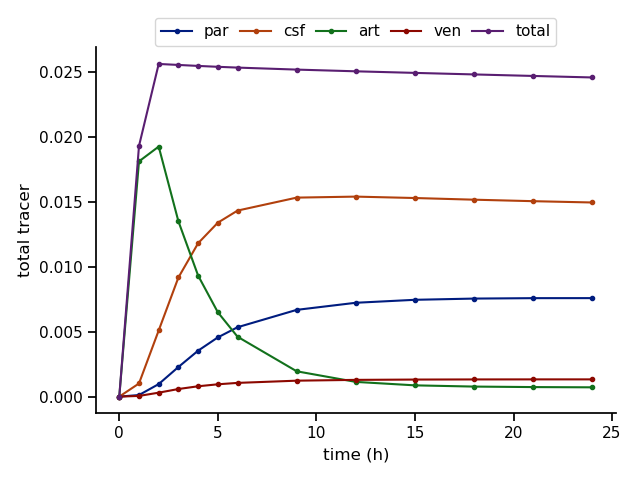
\includegraphics[width=\textwidth]{modelA_total_conc.png}
         \caption{arterial inflow, pure diffusion}
         \label{fig:y equals x}
     \end{subfigure}
     \hfill
     \begin{subfigure}[b]{0.33\textwidth}
         \centering
         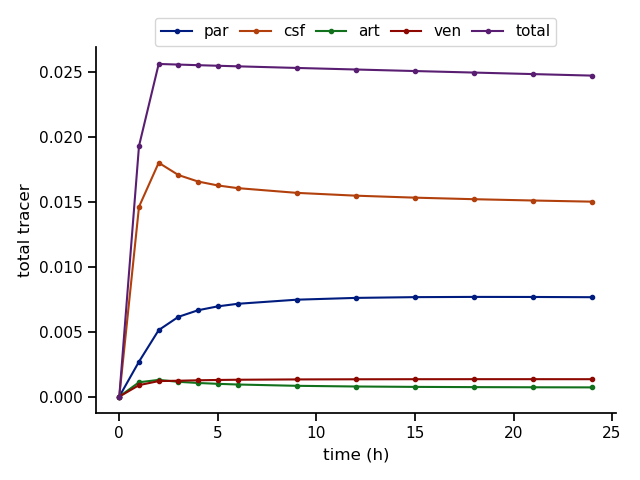
\includegraphics[width=\textwidth]{modelB_total_conc.png}
         \caption{SAS inflow, pure diffusion}
         \label{fig:three sin x}
     \end{subfigure}
     \hfill
     \begin{subfigure}[b]{0.33\textwidth}
         \centering
         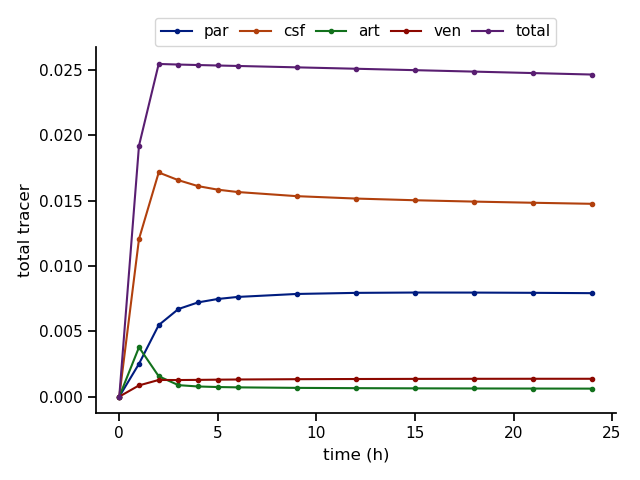
\includegraphics[width=\textwidth]{modelC_total_conc.png}
         \caption{arterial inflow, diffusion + PVS convection}
         \label{fig:five over x}
     \end{subfigure}
        \caption{Total tracer amount in parenchyma, CSF, arterial PVS and venous PVS}
        \label{fig:three graphs}
\end{figure}


\subsection*{Effect of interfaces (interface permeability)}

\begin{itemize}
    \item Model 0 (baseline): only diffusion, different diffusion coefficient in the parenchyma and SAS/PVS. No leak to vasculature (zero permeability). $\infty$ $\zeta_0$ at the PVS-SAS interface, $\zeta_1$ at the PVS-SAS interface. Koch et al could be a reference for PVS-parenchyma, maybe Tithof et al (2022, "A network model" ...) could give some ideas for parameters, also see Mestre et al, Nature comms, 2022. 
    \item 
    With altered interface permeabilities in the PVS (Model 1), and or in the parenchyma (Model 2) 
    \end{itemize}

\begin{figure}
    \caption{}
    \label{fig:1}
\end{figure}

\subsection*{Effect of convection}
\begin{itemize}
    \item 
    With convective flow in the PVS (zero flow in the parenchyma for now)
    \begin{itemize}
        \item 
        Model 3: PVS flow equal to 18.7 $\mu$m/s
        \item 
        Model 4: Better PVS flow (distributed, according to conservation of mass, assumptions on PVS area)
    \end{itemize}    
    \item 
    With convective flow in the ECS (out of scope here, for follow-up work?)
\end{itemize}

\begin{figure}
    \caption{}
    \label{fig:2}
\end{figure}
\subsection*{Effect of BBB}

Leakage to the blood, some sink/non-zero permeability for the PVS-blood (BBB) interface (Model N).

\begin{figure}
    \caption{}
    \label{fig:3}
\end{figure}

\subsection*{Effect of pia}
  
Effect of pia permeability (Model N-1)    

\begin{figure}
    \caption{}
    \label{fig:4}
\end{figure}


\section*{Discussion}

\subsection*{Limitations}

\begin{itemize}
    \item Pulsating brain. Natural to consider in follow-up work.
    \item PVS-blood exchange. Natural to consider in model variation here, or follow-up work.
    \item Accounting for brain diffusive anisotropy. Little effect expected. Maybe something to consider in small follow-up work.
\end{itemize}

\bibliography{references}

\newpage
\section*{Acknowledgements (not compulsory)}

Acknowledgements should be brief, and should not include thanks to anonymous referees and editors, or effusive comments. Grant or contribution numbers may be acknowledged.

\section*{Author contributions statement}

Must include all authors, identified by initials, for example:
A.A. conceived the experiment(s),  A.A. and B.A. conducted the experiment(s), C.A. and D.A. analysed the results.  All authors reviewed the manuscript. 

\section*{Additional information}

To include, in this order: \textbf{Accession codes} (where applicable); \textbf{Competing interests} (mandatory statement). 

The corresponding author is responsible for submitting a \href{http://www.nature.com/srep/policies/index.html#competing}{competing interests statement} on behalf of all authors of the paper. This statement must be included in the submitted article file.

\end{document}
